 %%%%%%%%%%%%%%%%%%%%%%%%%%%%%%%%%%%%%%%%%%%%%%%%%%%%%%%%%%%%%%%%%%%%%%%%%%%%%%%%
%2345678901234567890123456789012345678901234567890123456789012345678901234567890
%        1         2         3         4         5         6         7         8

\documentclass[letterpaper, 10 pt, conference]{ieeeconf}  % Comment this line out if you need a4paper

%\documentclass[a4paper, 10pt, conference]{ieeeconf}      % Use this line for a4 paper

\IEEEoverridecommandlockouts                              % This command is only needed if 
                                                          % you want to use the \thanks command

\overrideIEEEmargins                                      % Needed to meet printer requirements.

%In case you encounter the following error:
%Error 1010 The PDF file may be corrupt (unable to open PDF file) OR
%Error 1000 An error occurred while parsing a contents stream. Unable to analyze the PDF file.
%This is a known problem with pdfLaTeX conversion filter. The file cannot be opened with acrobat reader
%Please use one of the alternatives below to circumvent this error by uncommenting one or the other
%\pdfobjcompresslevel=0
%\pdfminorversion=4

% See the \addtolength command later in the file to balance the column lengths
% on the last page of the document

% The following packages can be found on http:\\www.ctan.org
\usepackage{graphicx} % for pdf, bitmapped graphics files
%\usepackage{epsfig} % for postscript graphics files
%\usepackage{mathptmx} % assumes new font selection scheme installed
%\usepackage{times} % assumes new font selection scheme installed
%\usepackage{amsmath} % assumes amsmath package installed
%\usepackage{amssymb}  % assumes amsmath package installed
\usepackage{amsmath}
\usepackage{algorithm}
\usepackage{algpseudocode}

\title{\LARGE \bf
 Non-linear Distributed MPC Coordination of Autonomous Vehicles using Optimality Condition Decomposition
}


\author{Marc Facerías$^{1}$, Vicenç Puig$^{2}$ and Alexandru Stancu$^{1}$% <-this % stops a space
\thanks{$^{1}$ M. Facerías and A. Stancu belong to the Faculty of Electrical Engineering,
        University of Manchester, The United Kingdom
        {\tt\small marc.faceriaspelegri@manchester.ac.uk}}%
\thanks{$^{2}$V. Puig belongs to the Institute of Robotics, CSIC-UPC, Barcelona
        Spain
        {\tt\small vicenc.puig@upc.edu}}%
}


\begin{document}



\maketitle
\thispagestyle{empty}
\pagestyle{empty}


%%%%%%%%%%%%%%%%%%%%%%%%%%%%%%%%%%%%%%%%%%%%%%%%%%%%%%%%%%%%%%%%%%%%%%%%%%%%%%%%
\begin{abstract}
In this paper, a novel non-linear distributed MPC coordination scheme for autonomous vehicles based on the Optimality Condition Decomposition (OCD) algorithm is proposed. 
As result, a local planner for each vehicle is obtained via the OCD application to the MPC coordination scheme is obtained for each vehicle, providing realistic paths to be executed in a collaborative manner. The proposed approach is able to determine paths that consider both individual goals and the environment so that agents can collaborate to safely navigate the studied environment. A case study in a ROS simulation environment is used to assess the validity of the proposed approach for real-time implementation.
\end{abstract}


%%%%%%%%%%%%%%%%%%%%%%%%%%%%%%%%%%%%%%%%%%%%%%%%%%%%%%%%%%%%%%%%%%%%%%%%%%%%%%%%
\section{Introduction}
\label{seq:Intro}
In the last few years, the automotive sector has been advancing more and more towards automatising transport systems, with autonomous cars being few years away from a general public adoption. In the new context of highly connected autonomous devices it is expected to see a paradigm shift, from the roads being streams of independent agents competing with each other to reach their goal to a flow of interconnected entities that seek to accomplish their objectives through peer to peer collaboration. Autonomous driving, and thus collaborative driving, can not be considered an unique problem, as there exists a wide range of scenarios that involve different behaviours. Consequently, current research is focused on solving individual sub-problems, such as intersection management \cite{Pei2021}, assistive driving \cite{medero2021control}, platooning \cite{Vlachos2022} or lane changes \cite{LaneChangeXie2021}, among others. 

This work focuses on treating the platooning problem in the domain of autonomous driving. We can differentiate two trends when studying collaborative navigation, depending on whether an optimisation problem is solved in a distributed or decentralised manner. On the one hand, decentralised techniques separate the systems via either estimations or relaxations of the coupling behaviours. On the other hand, distributed techniques rely on mathematical relaxations of the problem to solve it in a parallel iterative manner. 

Regarding distributed approaches, several research techniques are being developed to deal with collaborative navigation. For instance in \cite{DistriADMM}, the alternating direction method of multipliers (ADMM) algorithm is applied, being the main innovation with respect to other approaches the usage of a spline based characterisation of the environment. In similar lines of work, \cite{Vlachos2022} presents a platooning ADMM algorithm with a leader-follower structure and evaluates its performance in Carla, a high-fidelity simulator for autonomous driving. A distributed collision avoidance approach is presented in \cite{8550245}, where simple agents modelled through a double integrator are coordinated using ADMM and a linear approximation of the collision avoidance constraints that allow solving the problem in a simpler manner. Similarly, \cite{van2016online} presented an ADMM coordination strategy that relies on separating lines for obstacle avoidance and spline-based trajectory characterisation, showing how the distributed algorithm improved the results of its centralised counterpart. Moreover, distributed coordination strategies allow system reconfiguration in an ad-hoc manner, preventing local failures to compromise the whole system. An example of this behaviour can be found in \cite{adHoc2021}, where a novel online platoon reconfiguration technique is presented and compared to the current European standards, with an special focus on the physical limitations that need to be overcome to implement this family of algorithms. Following a different path, \cite{8648233} proposes an ADMM optimal consensus controller applied to systems of particles. Interestingly, some lines of work do not rely on optimising a common performance metric to force a collaborative nature. For instance, in \cite{Wang2015}, a game theoretic approach based on Gauss-Seidel iterative method is proposed, allowing agents to decide whether to compete or collaborate, achieving a more human-like behaviour while improving their performance compared with a classic MPC. In a similar line of work \cite{troullinos2021collaborative} proposes a coordinated graphs and Max-Plus algorithm to decide high level actions that agents should perform to rearrange themselves in a lane-free environment.

Alternatively, decentralised algorithms switch the paradigm and decouple each subsystem by ignoring their interactions or estimating optimisation variables of the neighbouring agents. In other words, they effectively assume that global performance is subject to maximising the performance of each individual in an isolated manner, leading to a competitive behaviour which opposes the collaborative nature of other architectures. For instance, in \cite{Hult2019} presents a decentralised solution for the navigation in road intersections where each agent acts individually and a second coordination layer gives priority to each of them in a centralised manner to minimise the cost related to its intersection. In another line of work, \cite{Lee2020} presents a platooning algorithm with an special focus on the physical implementation of the network with a real fleet of trucks following a leader. Similarly, \cite{Regragui2023} presents an urban navigation network where agents communicate with devices installed in the streets that assign plans seeking to optimise the routes in a collaborative manner. Other approaches rely on estimating the results of coupled sub-problems, as presented in \cite{mohseni2020distributed}, where an MPC structure is used along with compatibility constraints to decouple vehicles in shared environments. In general, this family of strategies tend to add external devices to the system to avoid degraded solutions which may appear due to the simplification of coupled dynamics, as presented in \cite{guillaume2008fast}. 

In this paper, a novel non-linear distributed MPC coordination scheme for autonomous vehicles based on the Optimality Condition Decomposition (OCD) algorithm is proposed. As result, a local planner for each vehicle is obtained via the OCD application to the MPC coordination scheme is obtained for each vehicle, providing realistic paths to be executed in a collaborative manner. The proposed approach is able to determine paths that consider both individual goals and the environment so that agents can collaborate to safely navigate the studied environment. A case study in a ROS simulation environment is used to assess the validity of the proposed approach for real-time implementation.

To the best of our knowledge OCD approach has not yet been considered in the context of a cooperative autonomous driving. Furthermore, while most of the literature require some sort of central coordination unit to either relax or coordinate the optimisation, we aim to solve in a fully distributed manner. 

The structure of the paper is the following: Section \ref{sec:statement} presents the problem statement and the OCD approach. Section \ref{seq:CaseStudy} shows the application of the proposed approach in the collaborative coordination of autonomous vehicles. Section \ref{sec:results} presents the simulation results in the considered case study scenario. Finally, Section \ref{sec:conclusions} draws the main conclusions and points several future research paths.

\section{Problem statement and proposed approach} \label{sec:statement}
\label{Sec:MA optimal plans}
\subsection{Problem statement}
The collaborative planning problem can be defined as the search of suitable paths for a group of autonomous vehicles (agents) that allow navigating an environment while satisfying a set of constraints (as e.g. collisions avoidance or road margins). These constraints vary depending on the nature of the system, being in this specific scenario the physical limits of the agents and the safety margins between them. The main complication associated with this type of problems is that in order to find a suitable path for each vehicle we need to embed all the agents of the system in a single optimisation problem, which may lead to idle times too big for any real time application. Furthermore, solving a single optimisation problem implies that the system needs a central computing unit and a communication network powerful enough to ensure the propagation of the solutions and retrieving of all the individual agent data.\\ 

The inherent fragility and inefficiency of the centralised approach motivated the reformulation of the problem in a distributed manner. Even though there is still a performance bottleneck related with the latency of the network, we can solve $N$ optimisation sub-problems locally while achieving an optimality degree close to the centralised case through the propagation of local solutions and solving the sub-problems iteratively until convergence. This approaches tend to present algorithm with a high computational load. Thus, an alternative can be found in decentralised optimization approaches, which are a relaxed version of the original problem that either ignore the coupling between subsystems or rely on an approximation of their local variables, leading to a set of $N$ independent problems. In this work, we are going to design our algorithm using the latter approach, and thus solving relaxed sub-problems to achieve global optimally in an iterative manner.

To derive this decentralised approach, in the next section the OCD method is introduced as a particular case of the Lagrangian relaxation methods.

% Solving the problem in a distributed fashion has a bigger computational cost involved, both in terms of communication burden and the optimisation time, but it provides a solution closer to its centralised counterpart considering a stopping criteria properly defined.On the other hand, decentralised approaches prioritise the computational time over the global performance of the system, sometimes leading to a poor global behaviour, but simplifying the overall structure of the algorithm. In this work we are going to design our algorithm using the latter approach, and thus solving relaxed sub-problems to achieve global optimally in an iterative manner.\\ 

\subsection{Lagrangian relaxation methods}
Lagrangian relaxation methods are techniques applied to optimisation problems that aim to solve a simplified relaxed version of the problem through the application of the Lagrange multipliers. In order to illustrate this concept, we will introduce an arbitrary optimisation problem in  Eq.\eqref{eq:LR example}.

\begin{equation}
\label{eq:LR example}
\begin{aligned}
    & \underset{x}{\text{min}} &&f(x) \\
    & \text{s.t.}\\
    & && h(x) \leq 0 \\
\end{aligned}
\end{equation}

We aim to relax   Eq.\eqref{eq:LR example} by adding the constraint $h(x)$ to the cost function through a term $\lambda$, known as a Lagrange multiplier, leading to $\underset{x}{\text{min}}f(x) + \lambda h(x)$.\\ 

It can be observed that the problem is enforced to minimise the term $\lambda h(x)$, which for an appropriate positive value of $\lambda$ is equivalent to treating $h(x)$ as a constraint. The same principle is exploited by several decomposition techniques, which take advantage of embedding certain coupling constraints as part of the cost function to solve the complete problem in a distributed manner. Even though there is a vast literature regarding the solution of this distributed problems, they can be classified as either Lagrangian decomposition or decentralised solution of the KKT conditions for local optimality \cite{kargarian2016toward}. Two of the most popular techniques are the ADMM and OCD, which belong to the first and second approaches, respectively. \\ 

It can be seen that among the literature presented in the introduction, ADMM is the most extended technique and, even though OCD is similar in essence, the latter presents some advantages that allow a system topology more convenient for the problem treated in this paper. As presented in \cite{Segovia2021}, the main advantage of OCD over ADMM is that the latter does require a central coordination unit to perform the dual variable update, while OCD only requires communication with peers that present coupling with each other. This key difference in the system structure not only avoids relying on a specific agent but opens the door to the implementation of security features and dynamic agent reallocation in a simpler manner. \\


As mentioned before, OCD is a technique based on the Lagrangian decomposition method, proposed in  \cite{conejo2006decomposition}, that aims to divide a complex problem into simpler sub-problems by separating the coupled constraints. In this context, consider an optimisation problem with two groups of variables $x = [x_1, x_2]$, as follows

\begin{equation}
\label{eq:OCD example}
\begin{aligned}
    & \underset{x_1,x_2}{\text{min}} &&f(x_1,x_2) \\
    & \text{s.t.}\\
    & && g_1(x_1)  \leq 0  \\
    & && g_2(x_2)  \leq 0 \\
    & && h_1(x_1,x_2)  \leq 0  \\
    & && h_1(x_1,x_2)  \leq 0 \\
\end{aligned}
\end{equation}
In this example, we consider $g_i$ separable constraints, which involve only one subset of states, while $h_i$ are constraints that do not allow a direct decomposition. This can be solved by fixing a certain subset of variables, leading to two problems of the following shape 
\begin{equation}
\label{eq:OCD Dexample}
\begin{aligned}
    & \underset{x_1}{\text{min}} &&f(x_1,\hat{x}_2)) + {\lambda_2} h_2(x_1,\hat{x}_2)\\
    & \text{s.t.}\\
    & && g_1(x_1)  \leq 0  \\
    & && h_1(x_1,\hat{x}_2)  \leq 0 \\
\end{aligned}
\end{equation}

For clarity purposes we will not write the second half of the distributed problem, as it can be obtained by switching indexes $1$ and $2$. 

By iterating through the update procedure in Algorithm \ref{alg:NL planning algorithm}, an approximation of the optimal solution is computed. It is worth to note that any update policy of $\alpha$ could be applied to improve the convergence rate of $\lambda$, but for simplicity purposes, a constant positive update rate has been used in this formulation. 
\begin{algorithm}[h]
\caption{Optimal Condition Decomposition}
\label{alg:NL planning algorithm}
\While{not convergence}
   \State Collect current $x_i$ and set $\hat{x}_i = x_i$
   \State Update ${\lambda_n} = {\lambda_n} + \alpha h(x^k_i,x^k_n)$
    \State Compute a step of $i_{th}$ optimisation problem
    \State Forward $x_n$ thorough the system
\EndWhile
\end{algorithm} 
\subsection {Non Linear DMPC formulation }
\label{NL MPC}
In order to propose a distributed control problem, its centralised counterpart is going to be presented, which in this case is equivalent to consider all the vehicles in the road and their interactions as a single system\\


\begin{equation}
\label{eq:opt problem}
\begin{aligned}
    & \underset{\Delta u^k_n}{\text{min}}  &&\mathrm{J}=\sum_{k=0}^{H} \sum_{n=0}^{N}( J^k_n(x^k_n)) \\
    % .....................
    & \text{s.t. } &&\forall k \in [0,H], \forall n \in [1,N]\\
    & && x^{k+1}_n = f(x^{k}_n,u^{k}_n)\\
    & && u^k_n = u^{k-1}_{n} + \Delta u^k_n \\ 
    & && u^k_n \in [\underline{u^k_n}, \overline{u^k_n} ] \\
    & && e_{y_{n}}^{k} \in [\underline{e_{y_{n}}^{k}}, \overline{e_{y_{n}}^{k}} ] \\
    % .....................
    &  &&\forall k \in [0,H], \forall n \in [1,N] ,\forall j \in [1,N]\ j \neq n\\
    & && g( p^{k}_j, p^{k}_j) \equiv \lVert p^{k}_n, p^{k}_j \rVert_2  \leq D_{sf} \\
\end{aligned}
\end{equation}

\noindent where $J^k_n(x^k_n)$ has the following quadratic shape:
\begin{equation}
    J^k_n(x^k_n) = xQx + \Delta u Q_u \Delta u + q_xx + q_uu + q_{\sigma}\sigma
\end{equation}

being $x$ is the vehicle state vector, $u$ the input vector, $e_{y_{i}}^{k}$ the lateral error and $\sigma$ a set of slack variables. $Q_x$, $Q_u$, $q_x$, $q_u$ and $q_{\sigma}$ are weighting factors applied to each variable, while $H$ and $N$ refer to the planning horizon and number of agents in the fleet, respectively. Obstacle avoidance constraints are represented by the term $g$ and formulated using the Euclidean distance, where $D_{sf}$ is the minimum allowed security distance. Finally, the vehicle model is an arbitrary function $f(x^{k}_n,u^{k}_n)$, which will be particularised in further sections of this paper.  \\ 

Applying OCD to Eq. \eqref{eq:opt problem} leads to $N$ subsystems of varying shape depending on their communication topology. In order to exemplify their structure we are going to present a simplified case with two agents $a_1$ and $a_2$. Eq. \eqref{eq:ego_agent} refers to $a_1$ while in Eq.\eqref{eq:slave_agent} refers to $a_2$. \\

\begin{equation}
\label{eq:ego_agent}
\begin{aligned}
    & \underset{u_k}{\text{min}} && \mathrm{J}=\sum_{k=0}^{H} ( J^k_1(x^k_1) + J^k_2(\hat{x}^k_2))\\
    & \text{s.t.} &&\forall k \in [0,H]\\
    & && x^{k+1}_1 = f(x^{k}_1,u^{k}_1)\\
    & && u^k_1 = u^{k-1}_{1} + \Delta u_1 \\ 
    & && u^k_1 \in [\underline{u^k_1}, \overline{u^k_1} ] \\
    & && e_{y_{1}}^{k} \in [\underline{e_{y_{1}}^{k}}, \overline{e_{y_{1}}^{k}} ] \\
    & && g(p^k_1,\hat{p}^k_2) \\

\end{aligned}
\end{equation}

\begin{equation}
\begin{aligned}
    \label{eq:slave_agent}
    & \underset{\Delta u^k_n}{\text{min}} && \mathrm{J}=\sum_{k=0}^{H} ( J^k_2(x^k_2) + J^k_1(\hat{x}^k_1))  + \lambda^k_{1,2}g(p^k_2,\hat{p}^k_1)\\
    % ........
    & \text{s.t.} &&\forall k \in [0,H]\\
    & && x^{k+1}_2 = f(x^{k}_2,u^{k}_2)\\
    & && u^k_2 = u^{k-1}_{2} + \Delta u^k_2 \\ 
    & && u^k_2 \in [\underline{u^k_2}, \overline{u^k_2} ] \\
    & && e_{y_{2}}^{k} \in [\underline{e_{y_{2}}^{k}}, \overline{e_{y_{2}}^{k}} ] \\
\end{aligned}
\end{equation}

As it can be seen, applying this formulation as presented in Eq. \eqref{eq:opt problem} leads to duplicated constraints. Specifically, when dealing with an arbitrary pair $i$ and $j$, two equivalent constraints are generated, as $g^{k,i,j} \equiv g^{k,j,i}$. In order to prevent it, we can apply the following heuristics:     
    
    \begin{itemize}
        \item if $i<j$, we will consider $i$ as the ego vehicle and add the constraint $ g( p^{k}_i, \hat{p}^{k}_j)$ to its optimisation problem. Accordingly,  $\lambda^h_{1,2} g( \hat{p}^{k}_i, p^{k}_j)$ is added to the neighbouring agent $j$. 
        \item if $i>j$, we will consider $j$ as the ego, treating the constraints in the same manner already presented, but inverting the roles of $i$ and $j$. 
    \end{itemize}
    
Additionally, slack variables $\sigma_u$, $\sigma_{e_y}$, $\sigma_g$, $\sigma_h$ were added to the system and introduced in the cost function with appropriate weighting factors. These variables allow the constraints associated to them to be violated, dramatically increasing the cost function value. Thus, this will only happen in situations that otherwise would lead to system deadlocks, e.g a bottleneck where the only way to advance is by being closer than $D_{sf}$. \\ 

\section{Coordination of autonomous vehicles}
\label{seq:CaseStudy}

The proposed approach presented in previous section will be used to deal with an environment where a group of $N$ agents enter a highway and rearrange themselves into a platooning formation. The system is rewarded to traverse the environment as close as possible to the maximum allowed velocity while keeping a safety distance between agents and respecting both the physical limits of the vehicle and the highway. Each vehicle is modelled after a scaled car and we consider that all members of the platoon have the same global path $G_p$, defined by a set of arc segments of length $l$ and curvature $k$, being $G_p = [l_0, k_0,l_1, k_1, ... , l_N, k_N]$.  Additionally, we consider no lanes present in the track, thus agents can position themselves in any formation as long as they remain within the road limits and keep inter-vehicular safety distance. Finally, each agent is assumed to follow local plans perfectly. While this assumption is not needed to assess the viability of the algorithm, it simplifies the experimental process and decouples possible control errors from the plans generated, which by design will be suitable for the agents. It is worth to mention that in strict theory, we could use the control actions generated by the MPC directly as the input of each individual in the platoon. However, due to the latency of the algorithm this would lead to poor performance. 

\subsection{System Modelling}
\label{sec:modeling}
% In this section the models of both the vehicle are the environment are introduced. Firstly, in \cite{sec:NL_model} the general non-linear model of an arbitrary agent of the system is presented. Secondly, in \cite{sec:LPV} the same model is presented in a pseudo-linear fashion. Finally, in \cite{sec:obs_avoidance} the model used to represent the interaction between agents is studied. 

\subsubsection{Non-linear vehicle model}
\label{sec:NL_model}

In this work, we opted to use a dual model, involving both Frenet frame coordinates and Cartesian coordinates. As discussed in \cite{Frenet2022}, both formulations have particular strengths, however models purely based on Frenet coordinates lack representing the vehicle physical insights necessary in autonomous driving, which motives proposing a mixed model. In this application, the variables associated to a Frenet frame are used to embed of the reference signal into the model via following a curvilinear reference defined by a curvature $k$ and an arc length $s$ at which the agent is located. On the other hand, we will add the terms related with the Cartesian positions and velocities, as they are adequate for collision checking, which is strongly related to the geometric disposition of the system. Furthermore, having access to $v_x$, $v_y$ and $w$ is critical from a performance point of view, as it allows adding comfort constraints. The Cartesian variables of the car model have been derived from a bicycle model, more information may be found in previous works developed within our research group \cite{alcala2020lpv}. A visual representation of both Frenet and Cartesian frames can be seen in Figure \ref{fig:FvC}. 
\begin{figure}
  \centering
  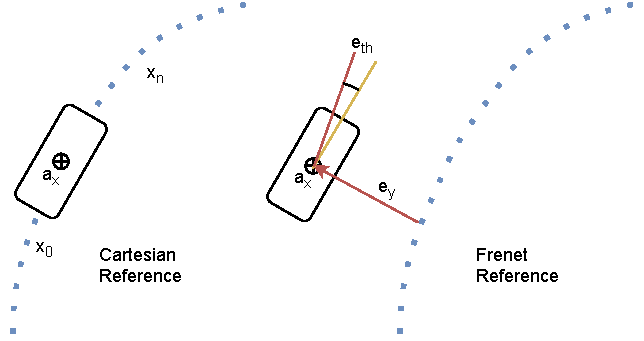
\includegraphics[width=0.75\columnwidth]{figs/FC.pdf}
    \caption{Two equivalent paths represented in both Cartesian and Frenet frames }
    \label{fig:FvC}
\end{figure}
\begin{equation}
    \label{eq:NL_model}
        \begin{aligned}
            &x = [v_x, v_y, \omega, x, y, \theta, s, e_y, \theta_e]\\ 
            &u = [\delta, a]
        \end{aligned}
\end{equation}
For clarity purposes, the continuous-time non-linear model will be presented as two sets of equations. Firstly, Eq. \eqref{eq:cartesian_dynamic_model} representing the Cartesian coordinates and secondly Eq. \eqref{eq:frenet_model} representing the Frenet frame coordinate set

\begin{subequations}
\label{eq:cartesian_dynamic_model}
\begin{equation}
    \begin{aligned}
       	& \dot v_x = a + \frac{- F_{yf} \sin{\delta} - \mu g}{m} + \omega v_y  \\
        & \dot v_y =  \frac{ F_{yf} \cos{\delta} + F_{yr}}{m} - \omega v_x \\
		& \dot \omega = \frac{ F_{yf} l_f \cos{\delta} - F_{yr} l_r}{I} \\
    	& \dot x = v_x \cos{\theta} - v_y \sin{\theta} \\
		& \dot y = v_x \sin{\theta} + v_y \cos{\theta} \\
        & \dot \theta = \omega \\
    	& \alpha_f = \delta - \tan^{-1} \left(  \frac{v_y}{v_x} - \frac{l_f \omega}{v_x} \right) \\
    	& \alpha_r = - \tan^{-1}  \left(  \frac{v_y}{v_x} + \frac{l_r \omega}{v_x} \right) \ , \
    \end{aligned}
\end{equation}
\noindent where
\begin{equation}   
	\label{eq:Pacejka_and_friction}
    \begin{aligned} 		
		&  F_{yf} = C_f \alpha_f \\
		&  F_{yr} = C_r \alpha_r \\      
    \end{aligned}
\end{equation}
\end{subequations}    

\noindent Cartesian state variables $v_x$, $v_y$ and $\omega$ represent the body frame velocities, i.e. linear in $x$, linear in $y$ and angular velocities, respectively. Accordingly, the position is defined by $x$, $y$, $\theta$ coordinates with respect to a global reference frame.
The variables $\delta$ and $a$ are the steering angle at the front wheels and the longitudinal acceleration vector on the rear wheels, respectively, and represent the inputs of the system.
$F_{yf}$ and $F_{yr}$ are the lateral forces produced in front and rear tires, respectively.
Front and rear slip angles are represented as $\alpha_f$ and $\alpha_r$, respectively, and $C_f$ and $C_r$ are the front and rear tire stiffness coefficients.
$m$ and $I$ represent the vehicle mass and inertia and $l_f$ and $l_r$ are the distances from the vehicle center of mass to the front and rear wheel axes, respectively. 

\begin{equation}
    \label{eq:frenet_model}
    \begin{aligned}
        & \dot s = \frac{v_x cos\theta_{e} - v_y sin\theta_{e}}{1 - e_{y} k } \\
		& \dot e_{y} = v_x \sin{\theta_{e}} + v_y \cos{\theta_{e}} \\
        & \dot \theta_{e} = \omega - \frac{v_x \cos{\theta_{e}} - v_y \sin{\theta_{e}} }{1 - e_{y} \kappa} \kappa \\
    \end{aligned}
\end{equation}
\noindent Frenet state variables are denoted as $s$, $e_{y}$ and $\theta_{e}$ and represent the position of the vehicle along the curve, the lateral error and the orientation error, respectively. Finally this model is particularised for a small scale vehicle by substituting the constants present in Table \ref{table:vehicle_parameters}.\\

\begin{table}
    \caption{Dynamic model parameters of the vehicle}
    \label{table:vehicle_parameters}
    \centering
    \begin{tabular}{ l|l||l|l }
    \hline
    Parameter & Value & Parameter & Value \\
    \hline
    \hline
    $l_f$       & 0.125  $m$    & $l_r$    & 0.125  $m$  \\
    $m$         & 1.98  $kg$   & $I$      & 0.06 $kg$ $m^2$  \\
    $C_f$       & 60            & $C_r$    & 60 \\
    $\mu$ 	    & 0.05          & $g$      & 9.81 $\frac{m}{s^2}$ \\      
    \hline
    \end{tabular}
\end{table}    

\subsubsection{Environment modelling}    

The reference to be followed by the platoon is modelled through a set of curvilinear segments of constant curvature $k$ and a given length $l$. This is embedded into the model by the time-varying constant $k$ and the state variables $s$, $e_{y}$ and $\theta_{e}$. In order to update the parameter $k$, a greedy search is performed through the set of curves seeking the one that encloses the current position of the vehicle, taking into account the Frenet frame state variables. By considering the previous position and taking into account that each segment has a constant curvature, we can perform this search locally without having a major impact on the algorithm computational time. Note that the correctness of $k$ is subject to the precision of the state variable $s$ which in a real scenario will depend on both the model quality and the onboard localisation module.\\

In this paper, it is assumed that the reference curves are computed offline, resembling what could be a segment of a highway. The same approach has been extensively used in the past, either by assuming prior knowledge of the track \cite{alcala2020lpv} or through an online estimation \cite{Kabzan2019}. However, it is not trivial to expand it to the autonomous driving domain, as shown in \cite{li2020fast}, the resulting Frenet curves may degrade in the presence of large road curvatures. It is worth to note that this is an active research line, being of special interest the algorithm proposed by \cite{Sun2020}, which allows to convert an arbitrary Cartesian reference into an usable curve while preventing this degradation. 


% ------------------------------------------------------------------------------
% ------------------------------------------------------------------------------

\section{Results}
\label{sec:results}
The effectiveness of the algorithm proposed in Section \ref{Sec:MA optimal plans} is going to be assessed by applying it under the conditions presented in Section \ref{sec:modeling}. The results of this section were generated using CASADI \cite{Casadi} and IPOPT \cite{wachter2006implementation} as a non-linear solver. The code was deployed in a ROS network where each agent acts as an individual computing thread, resembling a real network of autonomous agents. All the computing times presented in this section do not include communication delays, as they are negligible in the simulation platform. However, they should be taken into consideration for any practical implementation. Finally, all tests were carried out in a consumer laptop with 16Gb of RAM, an i7-13700H CPU and no specific hardware acceleration.\\ 

It is worth to note that solving the non-linear formulation is a NP-Hard problem \cite{nl_time}. Thus, results are susceptible to the experimental conditions. However, per definition, OCD will improve inaccurate solutions iteratively which can mitigate the workload by using non-optimal solutions of the sub-problems. The metrics used for the sake of the comparison are the 2D generated path, the safety limits, the look-ahead distance and the computational time per iteration.   In order to assess performance, we will use $v_x$ and both inter-vehicular and look-ahead distances. This selection is motivated by the fact that we aim to know how fast are we going to reach our goal and how safe is the trajectory going to be. It is trivial to see that higher linear velocities will lead to shorter trajectories. The selection of the safety metrics aims to represent how well can we react to unforeseen scenarios. Specifically, how far away can a detectable obstacle be to be considered in the plans and what margin do we have in the face of events such as an agent losing control of the vehicle or an animal crossing the road.\\

Firstly, as we can see in Figure \ref{fig:Vcomp}, agents maintain a velocity around the road limits, which in this case is set to $3$ m/s. A strict velocity profile may be enforced through modifying the cost function, but in this case it was treated as a soft objective.  In terms of the look-ahead distance, we can see how the inherent cost of a NL algorithm makes it prohibitive to plan considering further distances. In particular, we saw certain solution degradation when attempting longer planning horizons, so currently the paths are projected $0.625$ s which is roughly equivalent to $1.5$ m, being the look-ahead distance 5 times the length of our test vehicle. In terms of platoon performance, in Figure \ref{fig:FvC} it can be seen how vehicles rearrange into a formation that satisfies the minimum distance constraints, and advance along the center of track, reducing $e_y$. Note that this particular behaviour is enforced through the design of the cost function, as there is no other incentive of minimising the lateral error other than mimicking the expected human behaviour. Consequently, other arrangements could be incentivised through an appropriate cost function. 

\begin{figure}
  \centering
  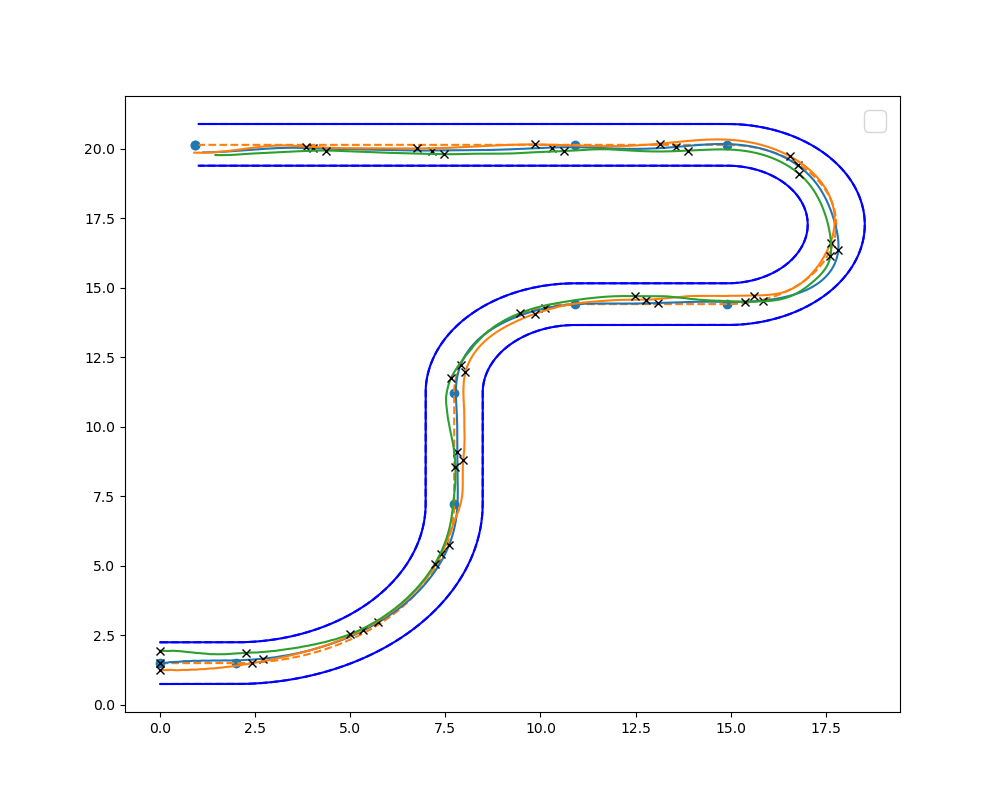
\includegraphics[width=\columnwidth]{figs/track_NL.png}
    \caption{Path traversed }
    \label{fig:FvC}
\end{figure}

\begin{figure}
  \centering
  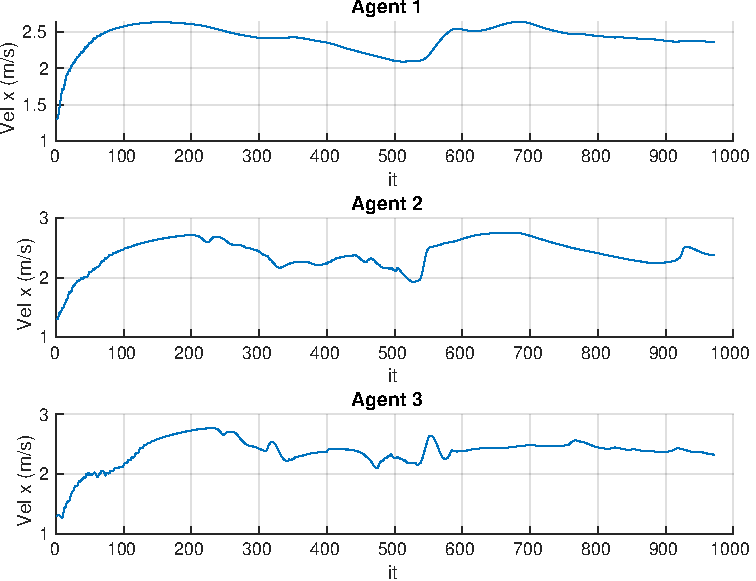
\includegraphics[width=\columnwidth]{figs/Cstates.pdf}
    \caption{Velocity profile }
    \label{fig:Vcomp}
\end{figure}

Finally, in terms of computational time and considering no communication delay we can see how the overall algorithm can be executed in under $500$ ms, which makes it feasible to scale it into a real device. Note that the first iteration is remarkably slower due to the computation of Hessian and Jacobian matrices used by IPOPT to solve the optimisation problem. However, this has no impact on the rest of the iterations as the solver is already warm started with suitable initial conditions, which are reasonably close to the expected optimal values.   \\ 

\begin{figure}
  \centering
  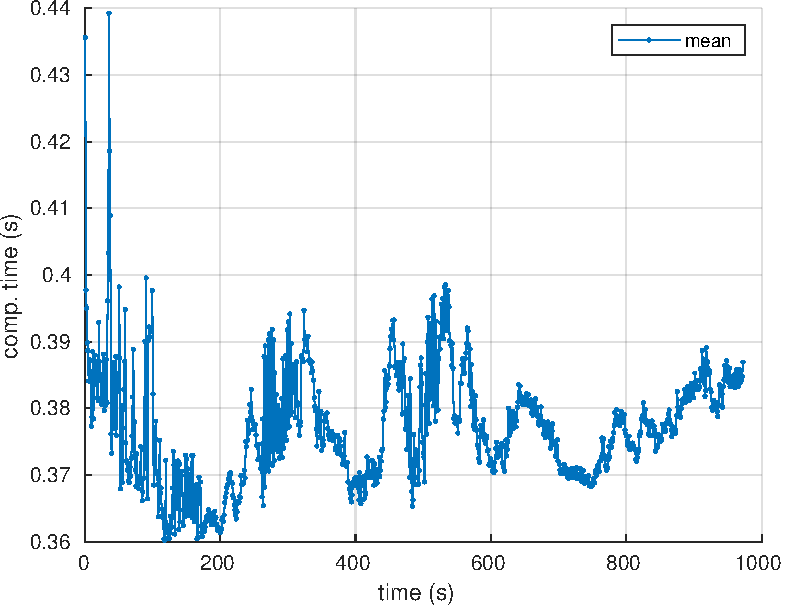
\includegraphics[width=\columnwidth]{figs/time.pdf}
    \caption{Average time along the agents}
    \label{fig:Tcomp}
\end{figure}

\section{Conclusions and future work}
\label{sec:conclusions} 

In this work, a novel non-linear distributed MPC coordination scheme for autonomous vehicles based on the Optimality Condition Decomposition (OCD) algorithm is proposed and tested it is viability in a shared environment. Furthermore, tests were implemented in a distributed manner as a ROS network, mimicking the physical layout of a platoon of autonomous vehicles, with agents reaching some sort of formation and stay in it while traversing the environment under some safety conditions, mimicking what can be understand to be non-competitive behaviour.\\  

Collaboration is still a key, if not mandatory, element in most autonomous driving situations where agents have individual goals and the environment forces individual agents to interact so that deadlocks and collisions are prevented. However, in this preliminary set of experiments we did not explore complex interactions, it remains uncertain how the proposed approach is to situations were some sort of negotiation is required to overcome the environment. For that reason, we aim to expand the algorithm presented in this paper by exploring other applications of OCD.\\

Over the development of this work it has been seen how over-complicating the formulation leads to intractable, if not unsolvable, optimisation problems that have little to no application outside of simulated environments. As a consequence, we aim to expand this research by apply variations of the planner in a cascade fashion so that collaborative decisions, which tend to have an slower occurrence rate can be taken in a higher level, less constraining both in terms of model accuracy and computational time, while the local plans are computed by a faster distributed algorithm with an special focus on the physical distribution of the agents and its safety.
\bibliographystyle{IEEEtran}
\bibliography{cas-refs}
\end{document}
